\section{Interfaz lógica de \SI{5}{V} — Retardos de propagación}
 
\subsection{Retardos con tres valores de pull-up}
 
Se midió el retardo de propagación $t_{PHL}$ (apagado del LED $\rightarrow$ salida HIGH)
y $t_{PLH}$ (encendido del LED $\rightarrow$ salida LOW) para tres valores de resistencia
de \textit{pull-up}: $R_L = \SI{985}{\ohm}$, $\SI{9.7}{k\ohm}$ y $\SI{98}{k\ohm}$.
La señal de entrada fue una onda cuadrada de \SI{10}{kHz}, 50\% DC, con
$I_F=\SI{10}{mA}$.
 
% ---- Imagen representativa (985 ohms) ----
\begin{figure}[H]
    \centering
    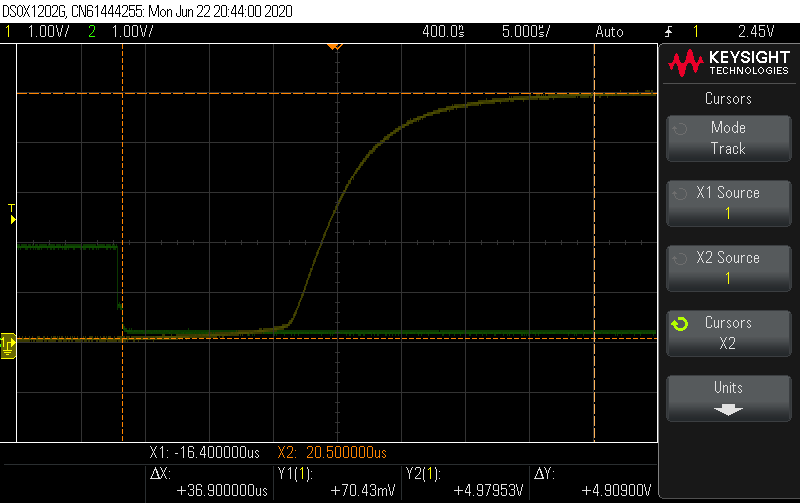
\includegraphics[width=0.7\linewidth]{img/Trise_R985.png}
    \caption{La señal amarrilla es la salida para $R_L=\SI{985}{\ohm}$ y la verde la entrada cuadrada.}
    \label{fig:osc_985}
\end{figure}
 
\begin{table}[H]
    \centering
    \begin{tabular}{
        S[table-format=6.0]
        S[table-format=3.1]
        S[table-format=4.1]
    }
        \toprule
        {$R_L$ (\si{\ohm})} & {$t_{PHL}$ (\si{\micro s})} & {$t_{PLH}$ (\si{\micro s})} \\
        \midrule
        985    &39.9 &2.2 \\
        9700   &168 &1.56 \\
        98000  &1668 &1.52 \\
        \bottomrule
    \end{tabular}
    \caption{Retardos de propagación.}
    \label{tab:retardos}
\end{table}
 
\noindent\textbf{Análisis:}
El retardo $t_{PLH}$ (salida subiendo de LOW a HIGH) aumenta con $R_L$ porque la
capacidad $C_{CE}$ del fototransistor se carga a través de $R_L$: a mayor resistencia,
mayor constante de tiempo $\tau = R_L C_{CE}$.  En cambio, $t_{PHL}$ (salida bajando)
depende principalmente del tiempo de descarga del transistor y varía poco con $R_L$,
en concordancia con la Fig.~12 del datasheet, donde $t_{PHL}$ es casi constante
($\approx \SI{2}{\micro s}$) mientras que $t_{PLH}$ crece aproximadamente en forma
logarítmica con $R_L$.
 
\subsection{Efecto de conectar la sonda en la base del optoacoplador}
 
Al conectar un canal del osciloscopio al terminal de base (pin~6) del 4N25, se introduce
la capacidad de entrada de la punta ($C_{sonda}\approx\SI{10}{pF}$ a \SI{1}{M\ohm}).  Esta
capacidad se suma a la capacitancia base-emisor del fototransistor interno, aumentando la
constante de tiempo de apagado y, en consecuencia, incrementando $t_{PLH}$.
Adicionalmente, la punta cierra un camino de descarga para la carga almacenada en la
base, lo que puede \emph{reducir} $t_{PHL}$ si provee una ruta de extracción de
portadores.  En la práctica se observa que $t_{PLH}$ aumenta notoriamente al colocar la
punta, mientras que $t_{PHL}$ cambia en menor medida.
 
\subsection{Efecto de la resistencia $R_{BE}$ — diferente ganancia}
 
Se conectó una resistencia $R_{BE}$ entre la base y el emisor del fototransistor.
Esta resistencia provee un camino de descarga continuo para los portadores
acumulados en la base, reduciendo el tiempo de saturación y por lo tanto $t_{PLH}$.
El efecto sobre el CTR es equivalente a reducir la ganancia efectiva del transistor:
\begin{equation}
    I_{C,\text{ef}} = \beta_{\text{ef}}\, I_{foto}, \qquad
    \beta_{\text{ef}} < \beta \text{ (sin } R_{BE}).
\end{equation}
 
\begin{figure}[H]
    \centering
    \begin{subfigure}[b]{0.48\linewidth}
        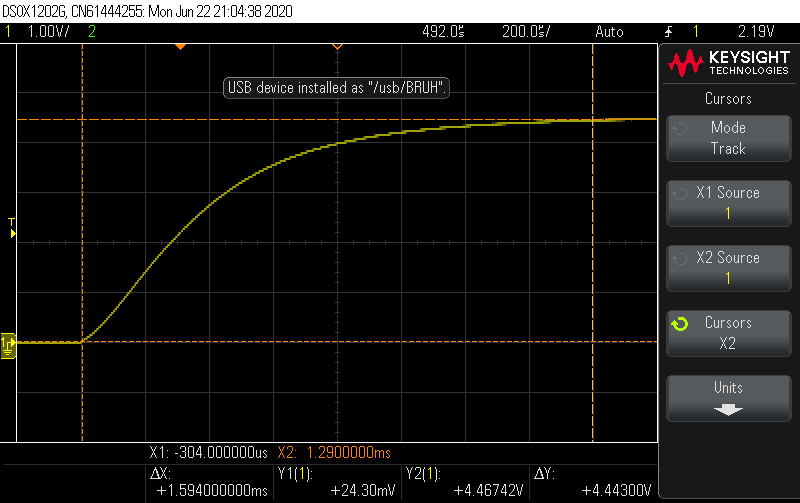
\includegraphics[width=\linewidth]{img/trise_sinRBE.png}
        \caption{Sin $R_{BE}$.}
    \end{subfigure}
    \hfill
    \begin{subfigure}[b]{0.48\linewidth}
        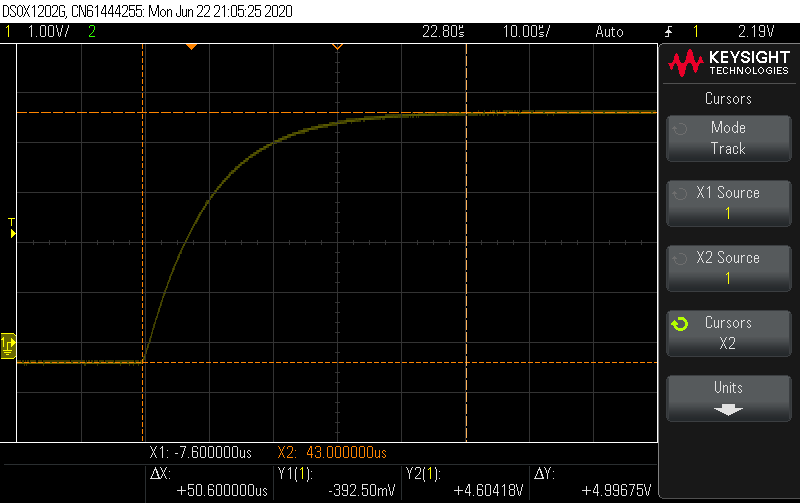
\includegraphics[width=\linewidth]{img/trise_conRBE.png}
        \caption{Con $R_{BE}$.}
    \end{subfigure}
    \caption{Comparación de $t_{PLH}$ con y sin $R_{BE}$ (misma $R_L$).}
    \label{fig:rbe_comp}
\end{figure}
 
\noindent Al agregar $R_{BE}$ el tiempo de subida $t_{PLH}$ disminuye apreciablemente
porque la carga almacenada en la base se evacua más rápido.  El precio es una caída del
CTR (menor corriente de colector para igual $I_F$), lo cual equivale a operar con una
ganancia menor, como refleja la curva normalizada del datasheet.